\documentclass[11pt, english]{article}
\usepackage{graphicx}
\usepackage[colorlinks=true, linkcolor=blue]{hyperref}
\usepackage[english]{babel}
\selectlanguage{english}
\usepackage[utf8]{inputenc}
\usepackage[svgnames]{xcolor}
\usepackage{svg}

\usepackage{listings}
\usepackage{afterpage}
\pagestyle{plain}

\definecolor{dkgreen}{rgb}{0,0.6,0}
\definecolor{gray}{rgb}{0.5,0.5,0.5}
\definecolor{mauve}{rgb}{0.58,0,0.82}

%\lstset{language=R,
%    basicstyle=\small\ttfamily,
%   stringstyle=\color{DarkGreen},
%    otherkeywords={0,1,2,3,4,5,6,7,8,9},
%    morekeywords={TRUE,FALSE},
%    deletekeywords={data,frame,length,as,character},
%    keywordstyle=\color{blue},
%    commentstyle=\color{DarkGreen},
%}

\lstset{frame=tb,
language=R,
aboveskip=3mm,
belowskip=3mm,
showstringspaces=false,
columns=flexible,
numbers=none,
keywordstyle=\color{blue},
numberstyle=\tiny\color{gray},
commentstyle=\color{dkgreen},
stringstyle=\color{mauve},
breaklines=true,
breakatwhitespace=true,
tabsize=3
}

\usepackage{here}


\textheight=21cm
\textwidth=17cm
%\topmargin=-1cm
\oddsidemargin=0cm
\parindent=0mm
\pagestyle{plain}

%%%%%%%%%%%%%%%%%%%%%%%%%%
% La siguiente instrucción pone el curso automáticamente%
%%%%%%%%%%%%%%%%%%%%%%%%%%

\usepackage{color}
\usepackage{ragged2e}

\global\let\date\relax
\newcounter{unomenos}
\setcounter{unomenos}{\number\year}
\addtocounter{unomenos}{-1}
\stepcounter{unomenos}
\gdef\@date{ Course \arabic{unomenos}/ 2019}

\begin{document}

\begin{titlepage}

\begin{center}
\vspace*{-1in}
\begin{figure}[htb]
\begin{center}
\centering
\begin{tabular}{@{}cccc@{}}
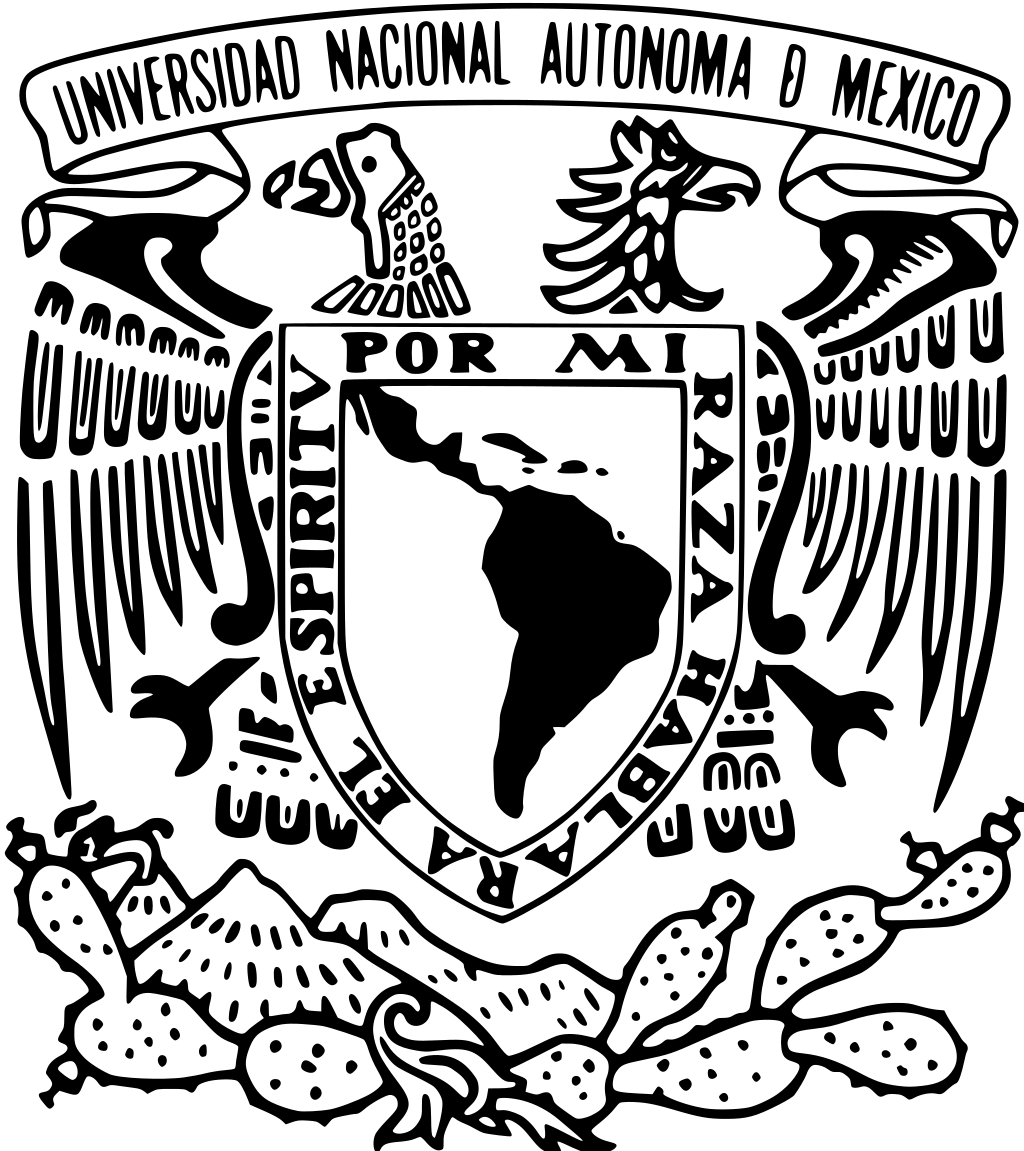
\includegraphics[width=6cm]{images/EscudoUNAM.png}
\hspace*{1.2in}

\includegraphics[width=6cm]{images/logoIng.png}
\end{tabular}
\end{center}
\end{figure}

FACULTAD DE INGENIERÍA - \@date\\
\vspace*{0.15in}
SECRETARÍA/DIVISIÓN: DIVISIÓN DE INGENIERÍA ELÉCTRICA \\
ÁREA/DEPARTAMENTO: INGENIERÍA EN COMPUTACIÓN \\
\vspace*{0.4in}
\begin{large}
LABORATORIO DE COMPUTACIÓN GRÁFICA E INTERACCIÓN HUMANO COMPUTADORA:\\
\end{large}
\vspace*{0.2in}
\begin{Large}
\textbf{Introducción a OpenGL} \\
\end{Large}
\vspace*{0.3in}
\vspace*{0.3in}
\begin{large}
Reynaldo Martell Avila \\
\end{large}
\vspace*{0.5in}
\vspace*{0.5in}
\begin{large}
\textbf{PRÁCTICA 2} \\
\end{large}
\end{center}
\end{titlepage}

\newcommand{\CC}{C\nolinebreak\hspace{-.05em}\raisebox{.4ex}{\tiny\bf +}\nolinebreak\hspace{-.10em}\raisebox{.4ex}{\tiny\bf +}}
\def\CC{{C\nolinebreak[4]\hspace{-.05em}\raisebox{.4ex}{\tiny\bf ++}}}

\tableofcontents

\newpage
\section{Objetivos de aprendizaje}
\subsection{Objetivos generales:}
El alumno aprenderá los conceptos básicos de OpenGL, el paradigma de programación y las funciones que se utilizan para renderizado de OpenGL.
\subsection{Objetivos específicos:}
El alumno aprenderá las funciones para el dibujo de primitivas geométricas en la pantalla, el paradigma de programación de OpenGL, a crear sus primeros Shaders de vértices y fragmentos, crear y utilizar el contexto de OpenGL, los conceptos de Vertex array object (VAO) y Vertex buffer object (VBO), así como la librería para crear ventanas y manejo de eventos.
\section{Recursos a emplear}
\subsection{Software}
Sistema Operativo: Windows 7
Ambiente de Desarrollo: Visual Studio 2017.
\subsection{Equipos}
Los equipos de cómputo con los que cuenta el laboratorio de Computación Gráfica
\subsection{Instrumentos}
\section{Fundamento Teórico}
\begin{itemize}
\item \textbf{Presentación de conceptos.} \\
Se le da a conocer al alumno los comandos \textbf{glGenVertexArrays}, \textbf{glBindVertexArray},
\textbf{glGenBuffers}, \textbf{glBindBuffer}, \textbf{glBufferData}, \textbf{glViewport}, nomenclatura de Vertex Shader,
Fragment Shader, agregar, compilar y verificar y usar shaders, e identificarlos como bloques
de información, se explica cuáles son los parámetros que pueden recibir estos comandos y
eso como afecta a lo dibujado. Posteriormente se utilizará los atributos de vértices usando
\textbf{glVertexAttribPointer}, \textbf{glEnableVertexAttribArray}.
\\
Finalmente se explican los comandos referentes a la creación de ventana 
\item \textbf{Datos necesarios.}
Librería OpenGL 3.3, librería de creación de ventanas, IDE de desarrollo (Visual Studio 2017.
\end{itemize}
\subsection{Desarrollo de actividades}
\begin{enumerate}
\item Navegar hasta el directorio de trabajo de la práctica pasada (Donde se clono el
repositorio), abrir un bash de git y teclear git pull origin master. Debe validar que
la actualización esté correcta.
\item Se explica el código base para para el uso de la librería GLFW y GLEW.
\item Se explica el uso de los eventos de los dispositivos convencionales mouse y
teclado (Sí es necesario).
\item Se muestra el ejemplo que crea un VAO, VBO, creación de un buffer y
transferencia de memoria a la GPU, se muestra como reciben los bloques de
memoria los Vertex shader y Fragment Shader.
\item Se muestra el uso los atributos de vértices, y los bloques de memoria.
\item Modificar el main.cpp para dibujar las siguientes
figuras, se deben usar dos VAOs y VBOs diferentes. Finalmente, con la tecla E
se muestra la estrella y con la tecla C la casa.
\begin{figure}[htb]
\begin{center}
\centering
\begin{tabular}{@{}cccc@{}}
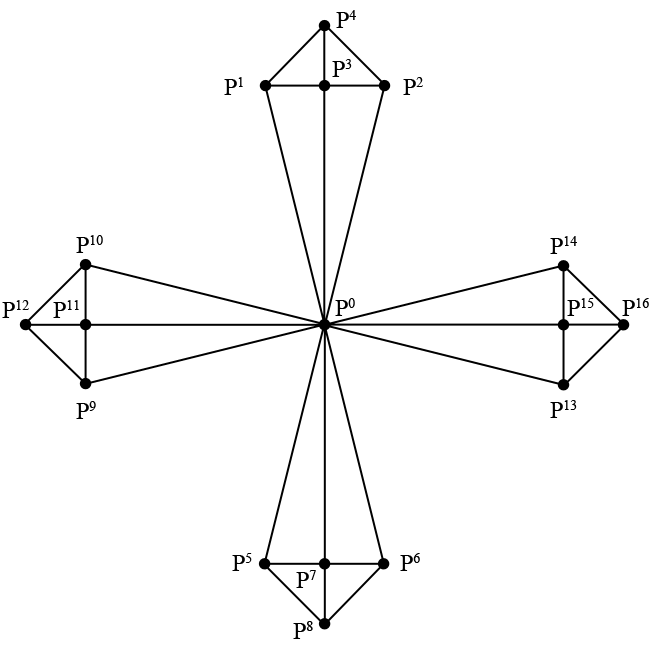
\includegraphics[width=5cm]{images/Estrella.png}
\hspace*{0.3in}
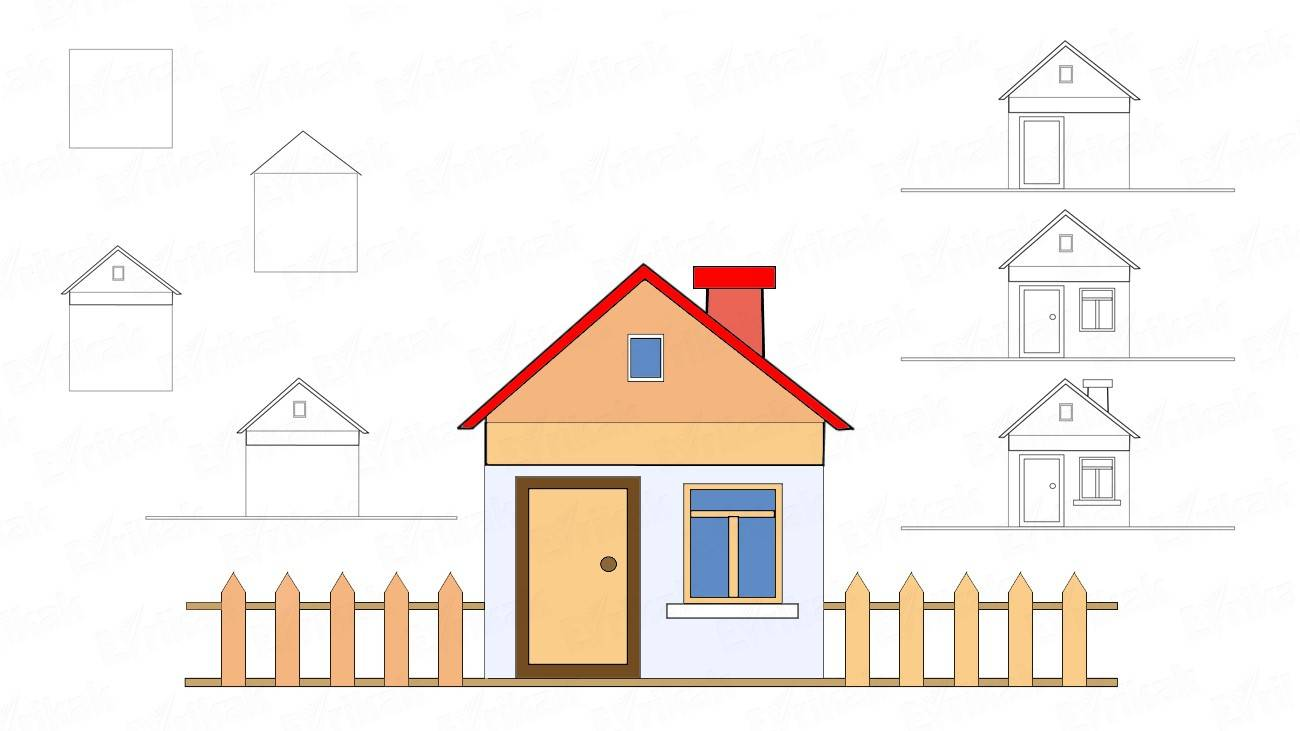
\includegraphics[width=7cm]{images/Casa.png}
\end{tabular}
\end{center}
\end{figure}
\item Se debe reportar y subir a github el ejercicio 6 anterior.
\end{enumerate}
\section{Observaciones y Conclusiones}
\section{Anexos}
\begin{enumerate}
\item Cuestionario previo.
\begin{enumerate}
\item ¿Qué es un polígono?
\item ¿Qué es un polígono convexo y cóncavo?
\item ¿Qué es un pixel?
\item ¿Qué es OpenGL?
\item ¿Qué es el contexto de OpenGL?
\item ¿Cuáles son las etapas básicas del pipeline de renderizado de OpenGL?
\item ¿Qué es un vertex shader?
\item ¿Qué es un fragment shader?
\item ¿Qué es un pixel?
\item ¿Qué son las NDC (Normalized device coordinates)
\end{enumerate}
\item Actividad de investigación previa.
\begin{enumerate}
\item ¿Qué es la resolución de un dispositivo?, investigue y anote la resolución del
monitor de su computadora principal.
\end{enumerate}
\end{enumerate}

%uoooooooooooooooo tumadreuooooooooooooooooooo UOOOOOOOOOOOOOOOOOOOOOOOOOOOOOOOOOOOOOOOOO
%AL FIN SE TERMINA ESTA PUTA MIERDA!!!!
%USEGREAS OSTOJEOGIRN ojeogiek


\end{document}